\section{Blind Attack}
\label{sec:blindattack}

In a real-world scenario, the key is typically unknown. Therefore we do not have any information whether our best candidate is correct or not. We need some rule to recognize a fairly good candidate, which we can then test for correctness by running AES encryption ourselves.

The most straightforward rule seems to be thresholding the gap of the best candidate, but it turns out that it is not that easy, see the following remark.

\begin{remark}
\label{rem:false}
	Especially note the attack against the \nth{1} byte using {\tt 3d} as a target and its last but one entry in Table~\ref{tab:lintargets} -- here an incorrect candidate has a gap of almost $26\%$. It is actually the largest gap of an incorrect candidate among all targets and all bytes using this particular instance of WBAES tables. (The largest gap of an incorrect candidate ever seen was almost $35\%$!)
	
	In our results, the target bits keep their original order (but reverse), therefore we can deduce the vector $B$ generating this particular target in terms of $T_B$ as introduced in Equation~\ref{eq:tba}. Here it is the second row of matrix of multiplication by $\texttt{3d}\pmod{x^8+1}$, see Example~\ref{ex:shiftmatrix}. Hence the vector is $B = 01011110$.
\end{remark}

In order to perform a blind attack, we studied our results deeper -- we were particularly interested in success rates of individual targets. The following section gives some of our remarks, next we suggest the blind attack itself in Section~\ref{sec:subblindattack}


% ==============================================================================
% ===   R E M A R K S                                                        ===
% ==============================================================================

\subsection{Remarks}
\label{sec:remarks}

We obviously cannot make conclusions based on a single {\tt KlinecWBAES} table instantiation only. In order to avoid specific behavior of a single instance, we created another $7$ instances. Then we acquired $1024$ traces and ran the attack against each of $16$ key bytes using all $255$ targets, for each instance. Altogether we ran $16\cdot255\cdot8=32\,640$ attacks, which, together with trace acquisition and filtering, took us several hours on a regular hardware.

We processed the results and displayed several statistics, here we present some of them. Note that we only considered strong candidates as introduced in Note~\ref{note:strong} (candidates with a gap greater than $10\%$).

The good news is that the overal success rate was $25\%$ (cf.\ $27\%$ and $31\%$ for our previous single-instance attack using the original SBox and Rijndael inverse, respectively), which gives us a hope that the new targets are successful, too. But our goal is to estimate rather individual success rate of each of our $255$ targets -- here the good news is that each target was successful at least once out of $16\cdot8=128$ chances.

Let us give the remarks now -- namely we present success rates of our targets, behavior of incorrect candidates, what happens if we use less than $1024$ traces, and finally we show a very peculiar result regarding leaking position within our traces.

\subsubsection{Success Rate of Individual Targets}
	
	Remind that we have $255$ targets and only $8$ independent\footnote{At the moment, we do not know which intermediate product leaks, hence cannot claim which values within single instance are independent. Clearly, more of them could be possibly independent.} instances of tables, which is quite a small data set for statistical purposes. For this reason, we rather group targets by different criteria and observe if they appear to be uniformly distributed. Note that we could possibly only refute uniformity this way, but it can still serve as reasonable justification.
	
	\paragraph{Group by corresponding $p$.}
	
	Here we make use of our former approach -- group the targets by corresponding $p$, and also study whether there is some influence of target invertibility; see the transfer in Section~\ref{sec:unify}. We put the results in a histogram, see Figure~\ref{fig:leaktargethist}. Here we give average percentual success rate together with its standard deviation (among $8$ measurements), for each group of targets. Invertible $p$'s are shown in green, non-invertible ones are orange.
	
	\begin{figure}[h]
	\begin{center}
		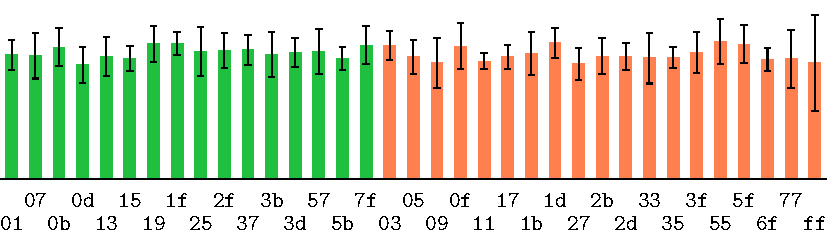
\includegraphics{figures/leak_target/leak_target.pdf}
		\caption{Average success rate and its standard deviation for targets grouped by corresponding $p$. Green represents invertible $p$'s, orange noninvertible ones.}
		\label{fig:leaktargethist}
	\end{center}
	\end{figure}
	
	Note that we did not give $y$-axis scale, since the only purpose is to distinguish uniform distribution, which appears to achieved be here.
	
	\paragraph{Group by fixed $4$ bits of $B$.}
	
	Another way of grouping we performed was grouping targets by fixing $4$ out of $8$ bits of their corresponding vector $B$. We fixed the first and the last $4$ bits and grouped them; see results in Figure~\ref{fig:leaktargetotherhist}, where these ways of grouping are given in green and orange, respectively. Note that group index can be computed as binary AND of mask {\tt 0xf0} and {\tt 0x0f} with vector $B$, respectively.
	
	\begin{figure}[h]
	\begin{center}
		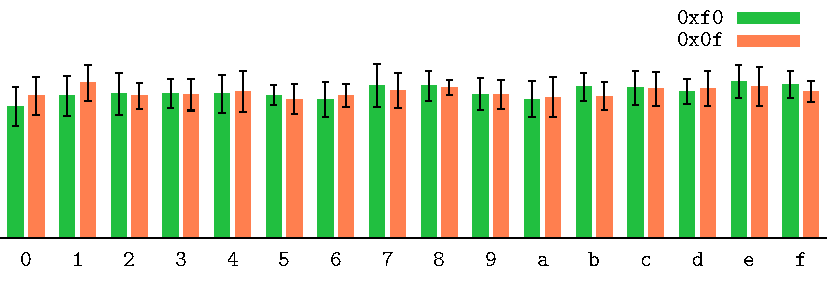
\includegraphics{figures/leak_target_other/leak_0x0f_0xf0.pdf}
		\caption{Average success rate and its standard deviation for targets grouped by fixed $4$ bits of corresponding vector $B$. Green represents fixed first $4$ bits, orange represents fixed last $4$ bits.}
		\label{fig:leaktargetotherhist}
	\end{center}
	\end{figure}
	
	\begin{remark}
	\label{rem:uniform}
		According to our previous observations, there does not seem to be a preferred target or a group of targets, therefore we will assume that success rate is uniform across all targets.
	\end{remark}

\subsubsection{Incorrect Candidates}
	
	There is an inconvenience, which emerges once we do not know the key -- we do not recognize the correct candidate anymore, see Remark~\ref{rem:false}. Therefore we will first observe behavior of incorrect ones in our self-controlled experiment where we know the key.
	
	\paragraph{Gaps of incorrect candidates.}
		
		Previously we defined a strong candidate as a candidate with a gap greater than $10\%$. Most strong candidates were correct, too, but there were a couple of exceptions, which we will refer to as {\em false positives}. In our overall results, $25\%$ of candidates were strong and correct, on the other hand, there were $11\%$ of false positives. On average, false positives had a gap of $14\%$ (cf.\ $40\%$ for correct ones) and the highest gap ever seen was $35\%$ (cf.\ $76\%$ for correct ones).
		
		A criterion based on thresholding might be on the one hand too strict, on the other hand, it might fail. Instead of looking for some well-balanced threshold, let us have a look at a much better observation about false positives, which will help us to distinguish them easily from the correct ones.
		% 1024:
		% strong & correct:
		% 	[1019, 1000, 978, 1008, 986, 1006, 1019, 999] => 1001.875 ... 24.6%
		% 	[39.46, 39.68, 39.5, 40.28, 40.2, 39.85, 39.86, 39.68] => 39.81375
		% strong & incorrect:
		% 	[442, 440, 425, 415, 433, 463, 413, 468] => 437.375 ... 10.7%
		% 	[14.05, 14.06, 14.16, 13.95, 14.26, 13.83, 14.0, 13.97] => 14.035
	
	\paragraph{Number of repetitions of false positives.}
		
		The good news is that the same false positive does not appear to repeat across targets very often. We observed the number of most repeating false positives across our $255$ targets and got the following results: on average, the number was $1.75$, the global maximum was $3$.
		
		Therefore having a candidate that repeats several times, we most likely have the correct candidate.
		% 	[1.88, 1.75, 1.81, 1.81, 1.62, 1.88, 1.62, 1.62]

\subsubsection{Using Less Traces}
	
	So far, we always used $1024$ traces in our attacks, let us have a look at results of the attack with much less traces. Note that Bos et al.\ \cite{bos2015differential} used $2000$ and $500$ traces for the attack targetting the original SBox and Rijndael inverse, respectively.
	
	Namely, we used $128$, $256$, $384$ and $512$ traces. For each number of traces, we attacked all of our $8$ instances of {\tt KlinecWBAES}, and observed ratios of strong candidates (both correct and incorrect) and their average gap; see results in Table~\ref{tab:ntraces}. Note that number of repeating false positives remains very low -- up to three.
	
	\begin{table}[H]
		\begin{center}
		\begin{tabular}{| c | c | c | c | c | c | c | c |}
			\hline
			Traces &    $128$ &    $256$ &    $384$ &    $512$ &    $1024$ \\
			\hline
			\hline
			Correct candidates
			       &  $9.8\%$ &   $17\%$ &   $20\%$ &   $21\%$ &    $25\%$ \\
			\hline
			Average gap of correct candidates
			       &   $24\%$ &   $32\%$ &   $35\%$ &   $37\%$ &    $40\%$ \\
			\hline
			\hline
			False positives
			       &  $7.7\%$ &   $11\%$ &   $12\%$ &   $12\%$ &    $11\%$ \\
			\hline
			Average gap of false positives
			       &   $13\%$ &   $14\%$ &   $14\%$ &   $14\%$ &    $14\%$ \\
			\hline
			\hline
			Reduced cost\tablefootnote{Reduced cost is to be introduced later.}
			       & $5\,400$ & $4\,700$ & $5\,500$ & $6\,400$ & $10\,500$ \\
			\hline
		\end{tabular}
		\end{center}
	\caption{Ratios of correct and incorrect candidates and their average gaps, for different numbers of traces.}
	\label{tab:ntraces}
	\end{table}
	
	% 128:
	% strong & correct:
	% 	[388, 420, 391, 411, 402, 393, 412, 397] => 401.750 ... 9.8%
	% 	[24.23, 24.39, 24.26, 23.65, 24.5, 24.01, 23.87, 23.65] => 24.07
	% strong & incorrect:
	% 	[262, 325, 351, 322, 309, 342, 285, 315] => 313.875 ... 7.7%
	% 	[13.34, 13.34, 13.13, 13.12, 12.9, 13.22, 13.26, 13.33] => 13.205
	
	% 256:
	% strong & correct:
	% 	[700, 670, 658, 722, 700, 709, 707, 683] => 693.625 ... 17.0%
	% 	[31.74, 32.49, 32.41, 31.83, 32.29, 31.31, 31.91, 32.11] => 32.01125
	% strong & incorrect:
	% 	[431, 472, 423, 441, 447, 451, 424, 482] => 446.375 ... 10.9%
	% 	[13.82, 13.85, 13.69, 14.1, 14.01, 14.1, 13.95, 14.36] => 13.985
	
	% 384:
	% strong & correct:
	% 	[814, 791, 784, 825, 790, 819, 812, 818] => 806.625 ... 19.8%
	% 	[35.84, 35.59, 35.14, 35.26, 36.19, 35.26, 35.77, 34.61] => 35.4575
	% strong & incorrect:
	% 	[491, 488, 484, 504, 487, 464, 509, 530] => 494.625 ... 12.1%
	% 	[14.17, 14.37, 13.97, 14.17, 14.14, 14.07, 14.23, 14.3] => 14.1775
	
	% 512:
	% strong & correct:
	% 	[879, 851, 855, 887, 848, 879, 881, 870] => 868.75 ... 21.3%
	% 	[37.25, 37.47, 36.58, 37.66, 38.04, 37.03, 37.42, 36.93] => 37.2975
	% strong & incorrect:
	% 	[471, 480, 473, 478, 472, 517, 432, 474] => 474.625 ... 11.6%
	% 	[14.02, 14.09, 13.96, 13.97, 14.23, 13.71, 14.29, 13.97] => 14.03

\subsubsection{Within-Trace Position of Leaks}
	
	Remind that our trace is a bit-wise serialization of least significant bytes of memory addresses, hence we can identify which bit within that byte was leaking -- simply by taking the leaking position within trace modulo $8$.
	
	\begin{note}
	\label{note:leakbit}
		This moduled position will be referred to as {\em leaking bit} (note the difference from target bit).
	\end{note}
	
	We noticed soon that leaking bits are not very well balanced as one would expect to, therefore we put this data into a histogram; see Figure~\ref{fig:leakbitall}. The histogram shows, for each leaking bit, the average number of strong correct candidates together with its standard deviation, which is surprisingly very low. Note that the histogram does not provide $y$-axis scale for similar reasons as for previous histograms.
	
	\begin{figure}[h]
	\begin{center}
		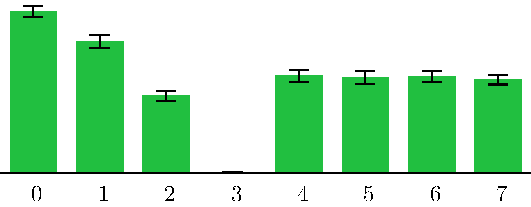
\includegraphics{figures/leak_bit/leak_bit.pdf}
		\caption{Average number of leaks and its standard deviation at each leaking bit.}
		\label{fig:leakbitall}
	\end{center}
	\end{figure}
	
	The \nth{0} and \nth{1} bits leaked slightly more, the \nth{2} bit slightly less than average, and the \nth{3} bit actually leaked only twice, while the overal average of the remaining bits was almost $160$! On the other hand, all of the remaining bits leaked fairly similarly. We do not have any explanation for this behavior, we only present it as our observation.


% ==============================================================================
% ===   B L I N D   A T T A C K   S U G G E S T I O N                        ===
% ==============================================================================

\subsection{Blind Attack Suggestion}
\label{sec:subblindattack}

\begin{note}
	This section only applies previous observations on a heuristic basis, there is no guarantee that our approach is the best.
\end{note}

In general, we suggest to use rather less traces, and repeat the attack with several targets until the sum of strong gaps of any candidate exceeds given bound. Let us choose reasonable values for both the number of traces and the bound.
\begin{description}
	\item[Number of traces.]
		In order to deduce a reasonable number of traces from results in Table~\ref{tab:ntraces}, let us introduce {\em reduced cost of gap}, defined as
		\begin{equation*}
			C(n, s, g) = \frac{n}{s\cdot g} ,
		\end{equation*}
		where $n$ stands for the number of traces, $s$ for average success rate and $g$ for average gap of a strong candidate.
		
		Note that this quantity corresponds with average time of the attack. Indeed, the more traces, the longer time; the better success rate or the bigger gap, the shorter time. Hence we can use this quantity to compare expected time of the attack using different number of traces.
		
		According to results in Table~\ref{tab:ntraces}, the best value of the reduced cost of gap was achieved for $256$ traces, therefore we suggest to use $256$ traces.
	\item[Bound.]
		According to our previous observation, false positives do not appear to repeat very much -- there were only a couple of repetitions for the most successful ones --, for less traces neither. Therefore we suggest to use $75\%$ as a cummulative bound, since it requires some $6$ hits for a fairly successful false positive, which appears to be hardly achievable.
\end{description}

\begin{remark}
\label{rem:attimpr}
	The attack can be further improved -- we can make the bound adaptive: we begin with a lower bound, obtain some (full) key candidate and verify it. Until the candidate is correct, we keep increasing the bound and merge our previous and new results. However, we did not implement this enhanced variant.
\end{remark}
